\section{Introduction}
\label{sec:introduction}

% state the learning objective 
The purpose of this laboratory assignment was to develop an AC/DC converter, using an envelope detector and a voltage regulator. The circuit we developed is shown in
 Figure~\ref{fig:circuit}.

We began by doing the simulation analysis of the circuit, trying out different configurations with the goal of understanding the problem and how the different 
parts of the circuit worked. After producing satisfactory results, we moved on to replicate the chosen circuit in the theoretical analysis, and subsequently compared the results side-by-side.
 These parts are described, respectively, in sections ~\ref{sec:simulation} and ~\ref{sec:analysis}. 

Finally, the conclusions of this study are indicated in
Section~\ref{sec:conclusion}.

\begin{figure}[ht] \centering
    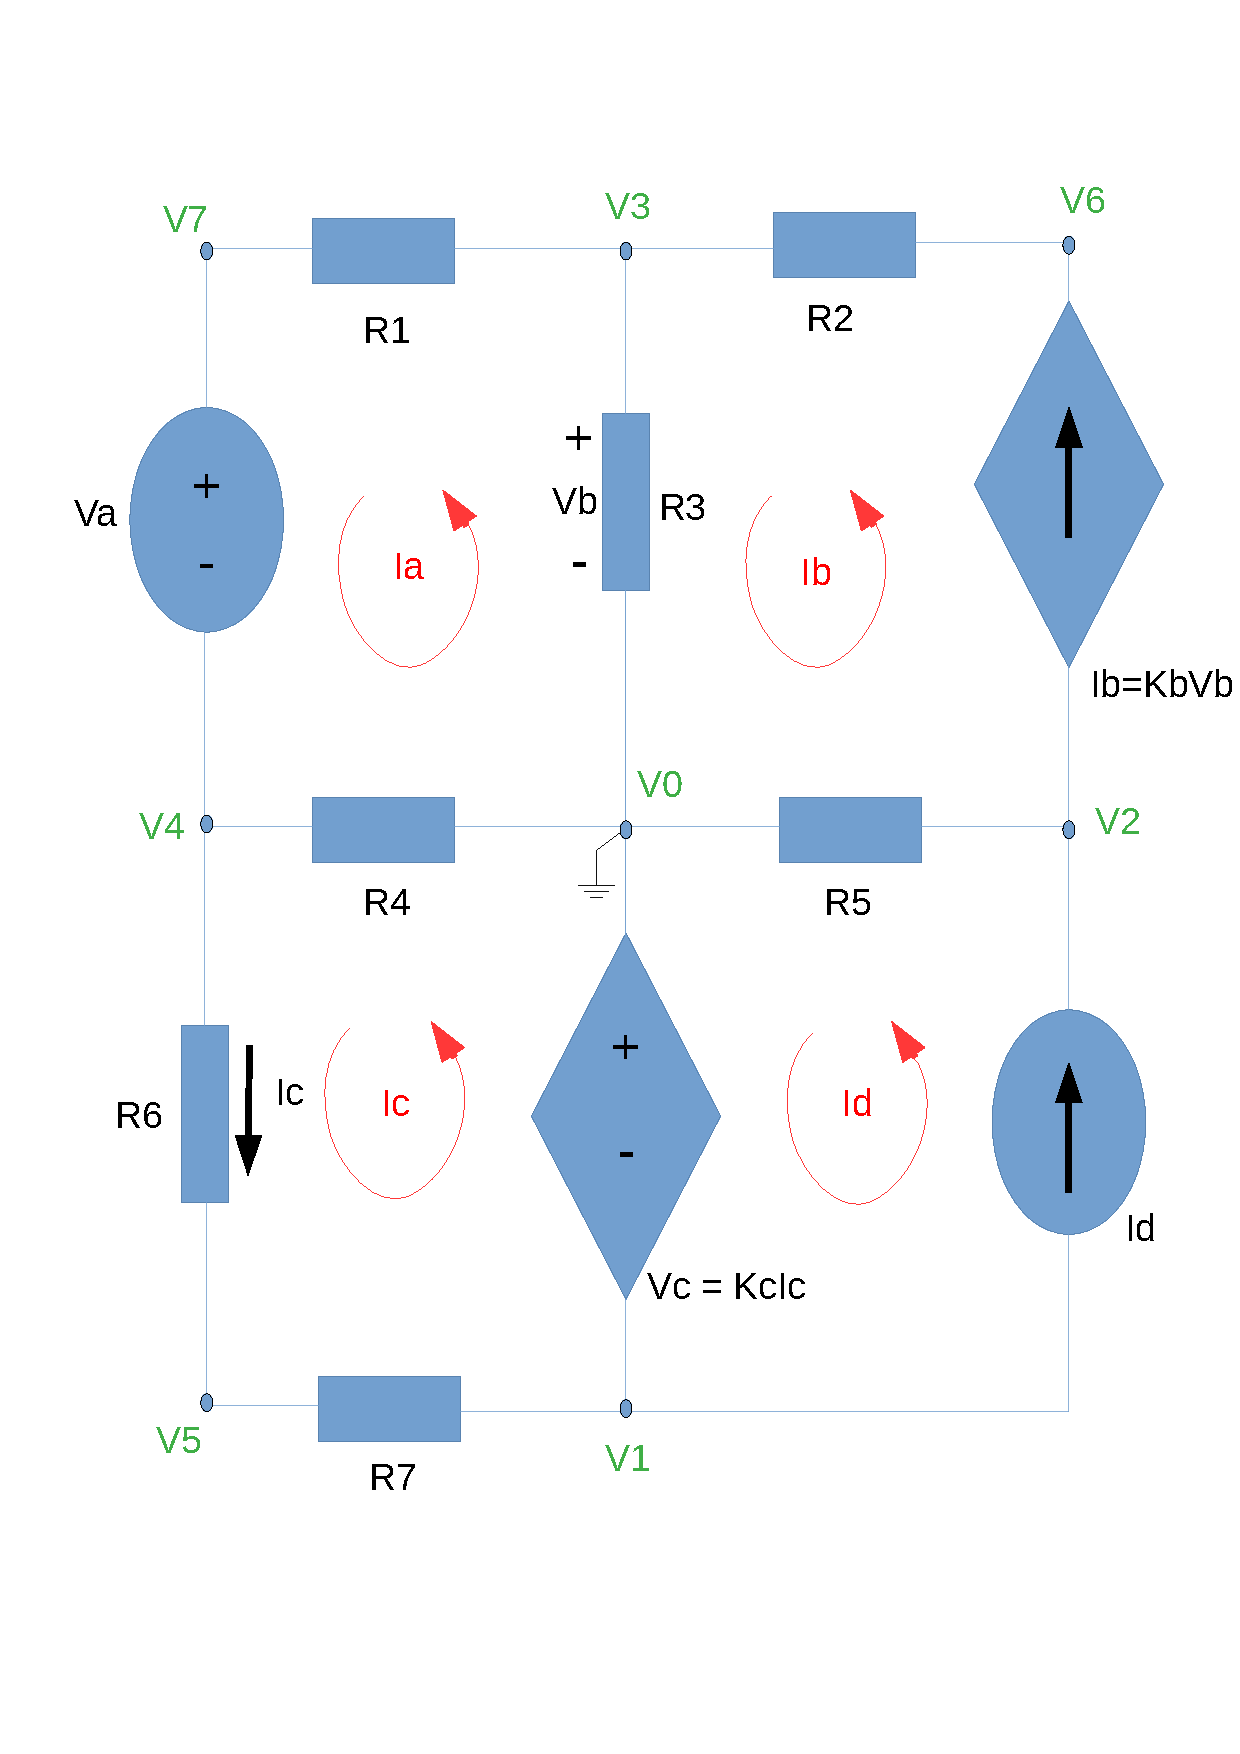
\includegraphics[width=0.4\linewidth]{circuito_tcfe.pdf}
    \caption{Circuit}
    \label{fig:circuit}
\end{figure}

